% Chapter 4: Seminar - SARIMA Models
% Harvard-quality academic presentation
% Bachelor program, Bucharest University of Economic Studies

\documentclass[9pt, aspectratio=169, t]{beamer}

% Ensure content fits on slides
\setbeamersize{text margin left=8mm, text margin right=8mm}

%=============================================================================
% THEME AND STYLE CONFIGURATION
%=============================================================================
\usetheme{default}
% Using default theme for clean header/footer control

% Color Palette (matching Redispatch PDF)
\definecolor{MainBlue}{RGB}{26, 58, 110}
\definecolor{AccentBlue}{RGB}{26, 58, 110}
\definecolor{IDAred}{RGB}{205, 0, 0}
\definecolor{DarkGray}{RGB}{51, 51, 51}
\definecolor{MediumGray}{RGB}{128, 128, 128}
\definecolor{LightGray}{RGB}{248, 248, 248}
\definecolor{VeryLightGray}{RGB}{235, 235, 235}
\definecolor{KeynoteGray}{RGB}{218, 218, 218}
\definecolor{SectionGray}{RGB}{120, 120, 120}
\definecolor{FooterGray}{RGB}{100, 100, 100}
\definecolor{Crimson}{RGB}{220, 53, 69}
\definecolor{Forest}{RGB}{46, 125, 50}
\definecolor{Amber}{RGB}{181, 133, 63}
\definecolor{Orange}{RGB}{230, 126, 34}
\definecolor{Purple}{RGB}{142, 68, 173}

% Gradient background (exact Keynote 315° gradient: white to RGB 218,218,218)
\setbeamertemplate{background}{%
    \begin{tikzpicture}[remember picture, overlay]
        \shade[shading=axis, shading angle=315,
        top color=white, bottom color=KeynoteGray]
        (current page.south west) rectangle (current page.north east);
    \end{tikzpicture}%
}
% Fallback solid color for compatibility
\setbeamercolor{background canvas}{bg=}

\setbeamercolor{palette primary}{bg=MainBlue, fg=white}
\setbeamercolor{palette secondary}{bg=MainBlue!85, fg=white}
\setbeamercolor{palette tertiary}{bg=MainBlue!70, fg=white}
\setbeamercolor{structure}{fg=MainBlue}
\setbeamercolor{title}{fg=IDAred}
\setbeamercolor{frametitle}{fg=IDAred, bg=}
\setbeamercolor{block title}{bg=MainBlue, fg=white}
\setbeamercolor{block body}{bg=VeryLightGray, fg=DarkGray}
\setbeamercolor{block title alerted}{bg=Crimson, fg=white}
\setbeamercolor{block body alerted}{bg=Crimson!8, fg=DarkGray}
\setbeamercolor{block title example}{bg=Forest, fg=white}
\setbeamercolor{block body example}{bg=Forest!8, fg=DarkGray}
\setbeamercolor{item}{fg=MainBlue}

% Footer colors (override Madrid theme blue)
\setbeamercolor{author in head/foot}{fg=FooterGray, bg=}
\setbeamercolor{title in head/foot}{fg=FooterGray, bg=}
\setbeamercolor{date in head/foot}{fg=FooterGray, bg=}
\setbeamercolor{section in head/foot}{fg=FooterGray, bg=}
\setbeamercolor{subsection in head/foot}{fg=FooterGray, bg=}

% Bullet styles (apply everywhere including blocks)
\setbeamertemplate{itemize item}{\color{MainBlue}$\boxdot$}
\setbeamertemplate{itemize subitem}{\color{MainBlue}$\blacktriangleright$}
\setbeamertemplate{itemize subsubitem}{\color{MainBlue}\tiny$\bullet$}
\setbeamertemplate{itemize/enumerate body begin}{\normalsize}
\setbeamertemplate{itemize/enumerate subbody begin}{\normalsize}

% Item spacing - compact style
\setlength{\leftmargini}{10pt}       % Level 1: minimal indent
\setlength{\leftmarginii}{10pt}      % Level 2: minimal additional indent
% Compact list spacing (zero extra space before/after lists in blocks)
\makeatletter
\def\@listi{\leftmargin\leftmargini \topsep 0pt \parsep 0pt \itemsep 0pt}
\def\@listii{\leftmargin\leftmarginii \topsep 0pt \parsep 0pt \itemsep 0pt}
\makeatother

\setbeamertemplate{navigation symbols}{}

%=============================================================================
% CUSTOM HEADLINE
%=============================================================================
\setbeamertemplate{headline}{%
    \vskip10pt%
    \hbox to \paperwidth{%
        \hskip0.5cm%
        {\small\color{FooterGray}\renewcommand{\hyperlink}[2]{##2}\insertsectionhead}%
        \hfill%
        \textcolor{FooterGray}{\small\insertframenumber}%
        \hskip0.5cm%
    }%
    \vskip4pt%
    {\color{FooterGray}\hrule height 0.4pt}%
}

%=============================================================================
% CUSTOM FOOTER
%=============================================================================
\usepackage{fontawesome5}

\setbeamertemplate{footline}{%
    {\color{FooterGray}\hrule height 0.4pt}%
    \vskip4pt%
    \hbox to \paperwidth{%
        \hskip0.5cm%
        \textcolor{FooterGray}{\small Time Series Analysis and Forecasting}%
        \hfill%
        \raisebox{-0.1em}{%
            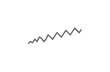
\begin{tikzpicture}[x=0.08em, y=0.08em, line width=0.4pt]
                \draw[FooterGray] (0,3) -- (1,4) -- (2,3.5) -- (3,5) -- (4,4) -- (5,6) -- (6,5.5) -- (7,4) -- (8,5) -- (9,7) -- (10,6) -- (11,5) -- (12,6.5) -- (13,8) -- (14,7) -- (15,6) -- (16,7.5) -- (17,9) -- (18,8) -- (19,7) -- (20,8.5) -- (21,10) -- (22,9) -- (23,8) -- (24,9.5);
            \end{tikzpicture}%
        }%
        \hskip0.5cm%
    }%
    \vskip6pt%
}

%=============================================================================
% PACKAGES
%=============================================================================
\usepackage[utf8]{inputenc}
\usepackage[T1]{fontenc}
\usepackage[english]{babel}
\usepackage{amsmath, amssymb, amsthm}
\usepackage{mathtools}
\usepackage{bm}
\usepackage{tikz}
\usetikzlibrary{arrows.meta, positioning, shapes, calc, decorations.pathreplacing, shadings}
\usepackage{booktabs}
\usepackage{multirow}
\usepackage{array}
\usepackage{graphicx}
\usepackage{hyperref}
\usepackage{colortbl}
\hypersetup{colorlinks=true, linkcolor=MainBlue, urlcolor=MainBlue}
\graphicspath{{../../logos/}{../../charts/}}
\hfuzz=2pt  % Suppress tiny overfull warnings (<2pt)
\vfuzz=2pt  % Suppress tiny vertical overfull warnings (<2pt)

%=============================================================================
% QUANTLET COMMAND
%=============================================================================
\newcommand{\quantlet}[2]{%
    \hfill\href{#2}{%
        \raisebox{-0.15em}{\includegraphics[height=0.7em]{ql_logo.png}}%
        \textcolor{MainBlue}{\tiny\ #1}%
    }%
}

%=============================================================================
% THEOREM ENVIRONMENTS
%=============================================================================
\theoremstyle{definition}
\setbeamertemplate{theorems}[numbered]
\newtheorem{defn}{Definition}
\newtheorem{thm}{Theorem}
\newtheorem{prop}{Proposition}
\newtheorem{rmk}{Remark}

%=============================================================================
% CUSTOM COMMANDS
%=============================================================================
\newcommand{\E}{\mathbb{E}}
\newcommand{\Var}{\text{Var}}
\newcommand{\Cov}{\text{Cov}}
\newcommand{\Corr}{\text{Corr}}
\newcommand{\R}{\mathbb{R}}
\newcommand{\N}{\mathbb{N}}
\newcommand{\Z}{\mathbb{Z}}
\newcommand{\RMSE}{\text{RMSE}}
\newcommand{\MAE}{\text{MAE}}
\newcommand{\MAPE}{\text{MAPE}}

% Quiz styling
\newcommand{\correct}{\textcolor{Forest}{\checkmark}}
\newcommand{\incorrect}{\textcolor{Crimson}{\texttimes}}

%=============================================================================
% CUSTOM TITLE PAGE
%=============================================================================
\defbeamertemplate*{title page}{hybrid}[1][]
{
    \vspace{0.2cm}
    % Logos row - top header (with clickable links)
    \begin{center}
        \href{https://www.ase.ro}{\includegraphics[height=1.0cm]{ase_logo.png}}\hspace{0.3cm}%
        \href{https://theida.net}{\includegraphics[height=1.0cm]{ida_logo.png}}\hspace{0.3cm}%
        \href{https://blockchain-research-center.com}{\includegraphics[height=1.0cm]{brc_logo.png}}\hspace{0.3cm}%
        \href{https://www.ai4efin.ase.ro}{\includegraphics[height=1.0cm]{ai4efin_logo.png}}\hspace{0.3cm}%
        \href{https://ipe.ro/new}{\includegraphics[height=1.0cm]{acad_logo.png}}\hspace{0.3cm}%
        \href{https://www.digital-finance-msca.com}{\includegraphics[height=1.0cm]{msca_logo.png}}%
    \end{center}

    \vspace{0.6cm}

    % Main title with Q logos on sides (with clickable links)
    \begin{center}
        \begin{minipage}{0.1\textwidth}
            \centering
            \href{https://quantlet.com}{\includegraphics[height=1.1cm]{ql_logo.png}}
        \end{minipage}%
        \begin{minipage}{0.78\textwidth}
            \centering
            {\LARGE\bfseries\usebeamercolor[fg]{title}\inserttitle}

            \vspace{0.3cm}

            {\usebeamerfont{subtitle}\usebeamercolor[fg]{title}\insertsubtitle}
        \end{minipage}%
        \begin{minipage}{0.1\textwidth}
            \centering
            \href{https://quantinar.com}{\includegraphics[height=1.1cm]{qr_logo.png}}
        \end{minipage}
    \end{center}

    \vspace{0.6cm}

    % Authors (left aligned)
    \hspace{0.5cm}{\usebeamerfont{author}\insertauthor}

    \vspace{0.3cm}

    % Institute/Affiliations (left aligned)
    \hspace{0.5cm}\begin{minipage}[t]{0.9\textwidth}
        \raggedright\small\insertinstitute
    \end{minipage}
}

%=============================================================================
% TITLE INFORMATION
%=============================================================================
\title[Time Series Analysis]{Time Series Analysis and Forecasting}
\subtitle{Seminar 4: SARIMA Models}
\author[D.T. Pele]{Daniel Traian PELE}
\institute{Bucharest University of Economic Studies\\
IDA Institute Digital Assets\\
Blockchain Research Center\\
AI4EFin -- Artificial Intelligence for Energy Finance\\
Romanian Academy, Institute for Economic Forecasting\\
MSCA Digital Finance}
\date{}

\begin{document}

% Title page (no header/footer)
{
\setbeamertemplate{headline}{}
\setbeamertemplate{footline}{}
\begin{frame}
    \titlepage
\end{frame}
}

%=============================================================================
% SEMINAR OUTLINE
%=============================================================================
\section{Overview}

\begin{frame}{Seminar Outline}
    \textbf{\large Today's Activities:}

    \vspace{0.4cm}

    \begin{enumerate}
        \item[\textcolor{MainBlue}{\textbf{1.}}] \textbf{Review Quiz} --- Checking understanding of SARIMA concepts
        \vspace{0.15cm}
        \item[\textcolor{MainBlue}{\textbf{2.}}] \textbf{True/False Questions} --- Conceptual checks
        \vspace{0.15cm}
        \item[\textcolor{MainBlue}{\textbf{3.}}] \textbf{Practice Problems} --- Calculations with SARIMA
        \vspace{0.15cm}
        \item[\textcolor{MainBlue}{\textbf{4.}}] \textbf{Worked Examples} --- Real-world applications
        \vspace{0.15cm}
        \item[\textcolor{MainBlue}{\textbf{5.}}] \textbf{Real Data Analysis} --- Case study with airline data
        \vspace{0.15cm}
        \item[\textcolor{MainBlue}{\textbf{6.}}] \textbf{Discussion Topics} --- Practical applications
        \vspace{0.15cm}
        \item[\textcolor{MainBlue}{\textbf{7.}}] \textbf{Summary} --- Key takeaways
        \vspace{0.15cm}
        \item[\textcolor{MainBlue}{\textbf{8.}}] \textbf{AI-Assisted Exercises} --- Human vs.\ AI modeling
        \vspace{0.15cm}
        \item[\textcolor{MainBlue}{\textbf{9.}}] \textbf{Key Formulas} --- Essential SARIMA formulas
    \end{enumerate}
\end{frame}

%=============================================================================
% SECTION 1: REVIEW QUIZ
%=============================================================================
\section{Review Quiz}

\begin{frame}{Quiz 1: Seasonal Differencing}
    \begin{alertblock}{Question}
        For monthly data with annual seasonality, what does the operator $(1-L^{12})$ do?
    \end{alertblock}

    \vspace{0.15cm}

    \begin{enumerate}[A)]
        \item Takes 12 consecutive differences
        \item Computes $Y_t - Y_{t-12}$
        \item Averages over 12 months
        \item Removes the first 12 observations
    \end{enumerate}

    \vspace{0.2cm}
    \pause
    \begin{exampleblock}{Answer: B -- Computes $Y_t - Y_{t-12}$}
        {\small
        \textbf{Seasonal difference operator}:
        \vspace{-0.3cm}
        \[
        (1-L^{12})Y_t = Y_t - L^{12}Y_t = Y_t - Y_{t-12}
        \]
        \vspace{-0.3cm}

        \textbf{Example} (January sales): $Y_{Jan2025} - Y_{Jan2024}$

        \textbf{Effect}: Removes stable annual seasonal pattern

        \textbf{Note}: $(1-L^s)$ for any seasonal period $s$ (quarterly: $s=4$, weekly: $s=52$)
        }
    \end{exampleblock}
\end{frame}

\begin{frame}{Visual: Seasonal Difference}
    \begin{center}
        \includegraphics[width=0.92\textwidth, height=0.65\textheight, keepaspectratio]{ch4_def_seasonal_diff.pdf}
    \end{center}
    \vspace{-0.2cm}
    \small Seasonal differencing removes annual patterns by comparing same periods across years.
    \quantlet{TSA\_ch4\_def\_seasonal\_diff}{https://github.com/QuantLet/TSA/tree/main/TSA_ch4/TSA_ch4_def_seasonal_diff}
\end{frame}

\begin{frame}{Quiz 2: SARIMA Notation}
    \begin{alertblock}{Question}
        What does SARIMA$(1,1,1) \times (1,1,1)_{12}$ represent?
    \end{alertblock}

    \vspace{0.3cm}

    \begin{enumerate}[A)]
        \item 12 different ARIMA models
        \item ARIMA with 12 AR and 12 MA terms
        \item ARIMA(1,1,1) with seasonal ARIMA(1,1,1) at period 12
        \item A model requiring 12 years of data
    \end{enumerate}
\end{frame}

\begin{frame}{Quiz 2: Answer}
    \begin{exampleblock}{Answer: C -- ARIMA(1,1,1) with seasonal ARIMA(1,1,1) at period 12}
        \begin{center}
            \includegraphics[width=0.95\textwidth, height=0.55\textheight, keepaspectratio]{sem4_sarima_notation.pdf}
        \end{center}
        $(1-\phi_1 L)(1-\Phi_1 L^{12})(1-L)(1-L^{12})Y_t = (1+\theta_1 L)(1+\Theta_1 L^{12})\varepsilon_t$
    \end{exampleblock}
\end{frame}

\begin{frame}{Visual: SARIMA Model Structure}
    \begin{center}
        \includegraphics[width=0.92\textwidth, height=0.65\textheight, keepaspectratio]{ch4_def_sarima.pdf}
    \end{center}
    \vspace{-0.2cm}
    \small SARIMA combines regular ARIMA components with seasonal components at lag $s$.
    \quantlet{TSA\_ch4\_def\_sarima}{https://github.com/QuantLet/TSA/tree/main/TSA_ch4/TSA_ch4_def_sarima}
\end{frame}

\begin{frame}{Quiz 3: The Airline Model}
    \begin{alertblock}{Question}
        The ``airline model'' refers to SARIMA$(0,1,1) \times (0,1,1)_{12}$. How many parameters does it have (excluding variance)?
    \end{alertblock}

    \vspace{0.3cm}

    \begin{enumerate}[A)]
        \item 2 parameters
        \item 4 parameters
        \item 6 parameters
        \item 12 parameters
    \end{enumerate}
\end{frame}

\begin{frame}{Quiz 3: Answer}
    \begin{exampleblock}{Answer: A -- 2 parameters ($\theta_1$ and $\Theta_1$)}
        \begin{center}
            \includegraphics[width=0.95\textwidth, height=0.55\textheight, keepaspectratio]{sem4_airline_model.pdf}
        \end{center}
        \textbf{Airline model}: $(1-L)(1-L^{12})Y_t = (1+\theta_1 L)(1+\Theta_1 L^{12})\varepsilon_t$

        Remarkably fits many seasonal economic series (Box \& Jenkins, 1970)
    \end{exampleblock}
\end{frame}

\begin{frame}{Quiz 4: ACF of Seasonal Data}
    \begin{alertblock}{Question}
        For monthly data with strong seasonality, where would you expect to see significant ACF spikes?
    \end{alertblock}

    \vspace{0.3cm}

    \begin{enumerate}[A)]
        \item Only at lag 1
        \item Only at lag 12
        \item At lags 12, 24, 36, ...
        \item Randomly distributed
    \end{enumerate}

    \vspace{0.5cm}
    \pause
    \begin{exampleblock}{Answer: C -- At lags 12, 24, 36, ...}
        {\small
        \textbf{Intuition}: January 2024 is similar to January 2023, 2022, etc.

        \textbf{ACF pattern}: Spikes at lags $s, 2s, 3s, \ldots$ ($\rho_{12}, \rho_{24}, \rho_{36} \neq 0$)

        \textbf{Diagnostic}: Slow decay at seasonal lags $\Rightarrow$ $D=1$; Cutoff after lag $s$ $\Rightarrow$ $Q=1$
        }
    \end{exampleblock}
\end{frame}

\begin{frame}{Visual: Seasonality Patterns}
    \begin{center}
        \includegraphics[width=0.92\textwidth, height=0.65\textheight, keepaspectratio]{ch4_def_seasonality.pdf}
    \end{center}
    \vspace{-0.2cm}
    \small Seasonal patterns repeat at regular intervals (monthly, quarterly, etc.) and may be additive or multiplicative.
    \quantlet{TSA\_ch4\_def\_seasonality}{https://github.com/QuantLet/TSA/tree/main/TSA_ch4/TSA_ch4_def_seasonality}
\end{frame}

\begin{frame}{Quiz 5: Multiplicative Structure}
    \begin{alertblock}{Question}
        In SARIMA, what does ``multiplicative structure'' mean?
    \end{alertblock}

    \vspace{0.3cm}

    \begin{enumerate}[A)]
        \item The seasonal amplitude grows proportionally
        \item Regular and seasonal polynomials are multiplied
        \item We multiply the data by seasonal factors
        \item The model is estimated using multiplication
    \end{enumerate}

    \vspace{0.5cm}
    \pause
    \begin{exampleblock}{Answer: B -- Regular and seasonal polynomials are multiplied}
        {\small
        \textbf{Multiplicative SARIMA}: $\phi(L)\Phi(L^s)(1-L)^d(1-L^s)^D Y_t = \theta(L)\Theta(L^s)\varepsilon_t$

        \textbf{Example}: $(1-\phi_1 L)(1-\Phi_1 L^{12}) = 1 - \phi_1 L - \Phi_1 L^{12} + \phi_1\Phi_1 L^{13}$

        \textbf{Cross-term} $\phi_1\Phi_1 L^{13}$: Captures interaction between short and long dynamics
        }
    \end{exampleblock}
\end{frame}

\begin{frame}{Quiz 6: Seasonal vs Regular Differencing}
    \begin{alertblock}{Question}
        When would you apply both regular ($d=1$) and seasonal ($D=1$) differencing?
    \end{alertblock}

    \vspace{0.3cm}

    \begin{enumerate}[A)]
        \item When data has only a trend
        \item When data has only seasonality
        \item When data has both trend and seasonal non-stationarity
        \item Never -- they cancel each other
    \end{enumerate}

    \vspace{0.5cm}
    \pause
    \begin{exampleblock}{Answer: C -- Both trend and seasonal non-stationarity}
        {\small
        \textbf{Combined}: $W_t = (1-L)(1-L^{12})Y_t = Y_t - Y_{t-1} - Y_{t-12} + Y_{t-13}$

        \textbf{When needed}: ACF slow decay at lags 1,2,3... $\Rightarrow d=1$; at lags 12,24,36... $\Rightarrow D=1$

        \textbf{Examples}: Airline passengers, retail sales, energy demand
        }
    \end{exampleblock}
\end{frame}

\begin{frame}{Quiz 7: Detecting Seasonality from ACF}
    \begin{alertblock}{Question}
        The ACF of a monthly time series shows slow decay at lags 12, 24, and 36. What does this suggest?
    \end{alertblock}

    \vspace{0.3cm}

    \begin{enumerate}[A)]
        \item The series is stationary
        \item The series needs regular differencing only
        \item The series has a seasonal unit root requiring $D=1$
        \item The series is white noise
    \end{enumerate}
\end{frame}

\begin{frame}{Quiz 7: Answer}
    \begin{exampleblock}{Answer: C -- Seasonal unit root requiring $D=1$}
        \begin{center}
            \includegraphics[width=0.95\textwidth, height=0.55\textheight, keepaspectratio]{sem4_seasonal_acf.pdf}
        \end{center}
        \textbf{Left}: Stationary seasonal (fast decay at seasonal lags)

        \textbf{Right}: Seasonal unit root (slow decay $\Rightarrow$ need $D=1$)
    \end{exampleblock}
\end{frame}

\begin{frame}{Quiz 8: Multiplicative vs Additive Seasonality}
    \begin{alertblock}{Question}
        If the seasonal amplitude of a time series grows proportionally with the level, this indicates:
    \end{alertblock}

    \vspace{0.3cm}

    \begin{enumerate}[A)]
        \item Additive seasonality -- use $(1-L^s)$
        \item Multiplicative seasonality -- use $\log$ transformation
        \item No seasonality present
        \item Need for regular differencing only
    \end{enumerate}
\end{frame}

\begin{frame}{Quiz 8: Answer}
    \begin{exampleblock}{Answer: B -- Multiplicative seasonality, use $\log$ transformation}
        \begin{center}
            \includegraphics[width=0.95\textwidth, height=0.55\textheight, keepaspectratio]{sem4_mult_add.pdf}
        \end{center}
        \textbf{Multiplicative}: Seasonal amplitude grows with level (diverging lines)

        \textbf{Solution}: Apply $\log$ transformation before fitting SARIMA
    \end{exampleblock}
\end{frame}

\begin{frame}{Quiz 9: Seasonal Subseries Plot}
    \begin{alertblock}{Question}
        In a seasonal subseries plot, what indicates multiplicative seasonality?
    \end{alertblock}

    \vspace{0.3cm}

    \begin{enumerate}[A)]
        \item Lines for each month are parallel
        \item Lines for each month diverge (spread increases over time)
        \item All months have the same mean
        \item Lines are horizontal
    \end{enumerate}

    \vspace{0.5cm}
    \pause
    \begin{exampleblock}{Answer: B -- Lines diverge (spread increases over time)}
        {\small
        \textbf{Subseries plot}: Groups data by month, plots each month's values across years

        \textbf{Parallel} $\Rightarrow$ Additive; \textbf{Diverging} $\Rightarrow$ Multiplicative; \textbf{Horizontal} $\Rightarrow$ No trend

        \textbf{Action}: If multiplicative, apply $\log$ before fitting SARIMA
        }
    \end{exampleblock}
\end{frame}

\begin{frame}{Quiz 10: Invertibility in SARIMA}
    \begin{alertblock}{Question}
        For SARIMA$(0,1,1) \times (0,1,1)_{12}$ to be invertible, which condition must hold?
    \end{alertblock}

    \vspace{0.3cm}

    \begin{enumerate}[A)]
        \item $|\theta_1| < 1$ only
        \item $|\Theta_1| < 1$ only
        \item Both $|\theta_1| < 1$ and $|\Theta_1| < 1$
        \item No invertibility condition exists for MA models
    \end{enumerate}

    \vspace{0.5cm}
    \pause
    \begin{exampleblock}{Answer: C -- Both $|\theta_1| < 1$ and $|\Theta_1| < 1$}
        {\small
        \textbf{Invertibility}: All MA roots outside unit circle

        \textbf{Multiplicative MA}: $(1+\theta_1 L)(1+\Theta_1 L^{12})$

        \textbf{Roots}: Regular $|z| = |{-1}/{\theta_1}| > 1 \Leftrightarrow |\theta_1| < 1$; Seasonal $|\Theta_1| < 1$

        \textbf{Both} conditions required for overall invertibility!
        }
    \end{exampleblock}
\end{frame}

\begin{frame}{Quiz 11: HEGY Test}
    \begin{alertblock}{Question}
        The HEGY test is used to:
    \end{alertblock}

    \vspace{0.3cm}

    \begin{enumerate}[A)]
        \item Estimate SARIMA parameters
        \item Test for unit roots at different frequencies (trend and seasonal)
        \item Check residual normality
        \item Compare SARIMA models using information criteria
    \end{enumerate}

    \vspace{0.5cm}
    \pause
    \begin{exampleblock}{Answer: B -- Test for unit roots at different frequencies}
        {\small
        \textbf{HEGY test} (Hylleberg-Engle-Granger-Yoo, 1990):

        Tests at: Zero freq ($\omega = 0$) $\Rightarrow d = 1$; Nyquist ($\omega = \pi$); Seasonal $\Rightarrow D = 1$

        \textbf{Decision}: Reject all $\Rightarrow$ seasonal dummies; Don't reject seasonal $\Rightarrow$ seasonal differencing
        }
    \end{exampleblock}
\end{frame}

\begin{frame}{Quiz 12: Seasonal MA Identification}
    \begin{alertblock}{Question}
        After applying $(1-L)(1-L^{12})$, the ACF shows a single significant spike at lag 12 only (no spike at lag 1). The PACF decays at seasonal lags. This suggests:
    \end{alertblock}

    \vspace{0.3cm}

    \begin{enumerate}[A)]
        \item SARIMA$(0,1,0) \times (0,1,1)_{12}$
        \item SARIMA$(0,1,1) \times (0,1,0)_{12}$
        \item SARIMA$(1,1,0) \times (1,1,0)_{12}$
        \item SARIMA$(0,1,1) \times (0,1,1)_{12}$
    \end{enumerate}

    \vspace{0.5cm}
    \pause
    \begin{exampleblock}{Answer: A -- SARIMA$(0,1,0) \times (0,1,1)_{12}$}
        {\small
        \textbf{Pattern}: Regular lags -- no spikes in ACF/PACF; Seasonal lags -- ACF cuts off at $s$, PACF decays

        \textbf{Interpretation}: No regular MA ($q = 0$); Seasonal MA(1) indicated ($Q = 1$)

        \textbf{Model}: $(1-L)(1-L^{12})Y_t = (1 + \Theta_1 L^{12})\varepsilon_t$
        }
    \end{exampleblock}
\end{frame}

\begin{frame}{Quiz 13: Over-differencing}
    \begin{alertblock}{Question}
        After differencing, the ACF shows a large negative spike at lag 1 or lag $s$. This typically indicates:
    \end{alertblock}

    \vspace{0.3cm}

    \begin{enumerate}[A)]
        \item The model needs more AR terms
        \item The series has been over-differenced
        \item The series is perfectly stationary
        \item Heteroskedasticity is present
    \end{enumerate}

    \vspace{0.5cm}
    \pause
    \begin{exampleblock}{Answer: B -- The series has been over-differenced}
        {\small
        \textbf{Signature}: ACF at lag 1 $\approx -0.5$ $\Rightarrow$ over-diff at $d$; ACF at lag $s$ $\approx -0.5$ $\Rightarrow$ over-diff at $D$

        \textbf{Why?} $\Delta^2 Y_t = \varepsilon_t - \varepsilon_{t-1}$ is MA(1) with $\theta = -1$, giving $\rho_1 = -0.5$

        \textbf{Fix}: Reduce $d$ or $D$ by one and re-examine ACF/PACF
        }
    \end{exampleblock}
\end{frame}

\begin{frame}{Quiz 14: Forecasting Horizon}
    \begin{alertblock}{Question}
        For a SARIMA model with $D=1$, what happens to forecast confidence intervals as the horizon $h \to \infty$?
    \end{alertblock}

    \vspace{0.3cm}

    \begin{enumerate}[A)]
        \item They converge to a fixed width
        \item They grow without bound
        \item They shrink to zero
        \item They oscillate seasonally
    \end{enumerate}

    \vspace{0.5cm}
    \pause
    \begin{exampleblock}{Answer: B -- They grow without bound}
        {\small
        \textbf{Unit root property}: Any unit root causes unbounded forecast variance

        \textbf{For SARIMA with $D=1$}: $\Var(\hat{Y}_{T+h} - Y_{T+h}) \to \infty$ as $h \to \infty$

        \textbf{Intuition}: Seasonal shocks accumulate; long-range forecasts have wide CIs
        }
    \end{exampleblock}
\end{frame}

\begin{frame}{Quiz 15: Seasonal Period Selection}
    \begin{alertblock}{Question}
        You have daily data showing clear weekly patterns. What seasonal period $s$ should you use in a SARIMA model?
    \end{alertblock}

    \vspace{0.15cm}

    \begin{enumerate}[A)]
        \item $s = 12$ (monthly)
        \item $s = 7$ (weekly)
        \item $s = 365$ (yearly)
        \item $s = 24$ (hourly)
    \end{enumerate}

    \vspace{0.2cm}
    \pause
    \begin{exampleblock}{Answer: B -- $s = 7$ (weekly)}
        {\small
        \begin{center}
        \vspace{-0.2cm}
        \begin{tabular}{lll}
            \textbf{Data} & \textbf{Pattern} & \textbf{Period $s$} \\
            Daily & Weekly & 7 \\
            Monthly & Annual & 12 \\
            Quarterly & Annual & 4
        \end{tabular}
        \end{center}
        \vspace{-0.1cm}
        \textbf{Rule}: $s$ = observations per cycle of dominant pattern
        }
    \end{exampleblock}
\end{frame}

\begin{frame}{Quiz 16: Seasonal AR Component}
    \begin{alertblock}{Question}
        In the seasonal component $\Phi(L^s) = 1 - \Phi_1 L^s$, what does the coefficient $\Phi_1 = 0.8$ tell us?
    \end{alertblock}

    \vspace{0.3cm}

    \begin{enumerate}[A)]
        \item 80\% of this period's value comes from the previous period
        \item There is 80\% correlation between consecutive observations
        \item 80\% of this period's value is explained by the same period last year
        \item The seasonal pattern explains 80\% of variance
    \end{enumerate}

    \vspace{0.5cm}
    \pause
    \begin{exampleblock}{Answer: C -- 80\% explained by same period last year}
        {\small
        \textbf{SAR(1)}: $Y_t = \Phi_1 Y_{t-12} + \varepsilon_t$

        \textbf{With $\Phi_1 = 0.8$}: $Y_{Jan2024} = 0.8 \cdot Y_{Jan2023} + \varepsilon_t$

        \textbf{Interpretation}: Strong seasonal persistence -- 80\% explained by same month last year

        \textbf{Stationarity}: Requires $|\Phi_1| < 1$ (satisfied here)
        }
    \end{exampleblock}
\end{frame}

\begin{frame}{Quiz 17: Seasonal Stationarity}
    \begin{alertblock}{Question}
        A seasonal process with $\Phi_1 = 1$ in SARIMA$(0,0,0) \times (1,0,0)_{12}$ is:
    \end{alertblock}

    \vspace{0.3cm}

    \begin{enumerate}[A)]
        \item Stationary
        \item Has a seasonal unit root (seasonally integrated)
        \item Explosive
        \item Undefined
    \end{enumerate}

    \vspace{0.5cm}
    \pause
    \begin{exampleblock}{Answer: B -- Has a seasonal unit root}
        {\small
        \textbf{Model}: $Y_t = Y_{t-12} + \varepsilon_t$ (seasonal random walk)

        \textbf{Properties}: Variance grows with time; each month follows its own RW; need $D = 1$

        \textbf{Analogy}: Like regular random walk but at seasonal frequency
        }
    \end{exampleblock}
\end{frame}

\begin{frame}{Quiz 18: Model Comparison}
    \begin{alertblock}{Question}
        Model A: SARIMA$(1,1,1) \times (1,1,1)_{12}$ has AIC = 520. Model B: SARIMA$(0,1,1) \times (0,1,1)_{12}$ has AIC = 525. Which statement is most accurate?
    \end{alertblock}

    \vspace{0.3cm}

    \begin{enumerate}[A)]
        \item Model A is always better since it has lower AIC
        \item Model B should be preferred due to parsimony despite higher AIC
        \item The AIC difference of 5 suggests Model A is substantially better
        \item We cannot compare models with different orders
    \end{enumerate}

    \vspace{0.5cm}
    \pause
    \begin{exampleblock}{Answer: C -- AIC difference of 5 suggests Model A is substantially better}
        {\small
        \textbf{Rule of thumb}: $\Delta$AIC $< 2$: equivalent; $2$--$10$: some evidence; $> 10$: strong evidence

        \textbf{Here}: $\Delta$AIC $= 5$ suggests Model A meaningfully better

        \textbf{Always}: Also check residual diagnostics and forecast performance!
        }
    \end{exampleblock}
\end{frame}

\begin{frame}{Quiz 19: Seasonal Patterns in Residuals}
    \begin{alertblock}{Question}
        After fitting a SARIMA model, you notice significant ACF spikes at lags 12 and 24 in the residuals. What does this indicate?
    \end{alertblock}

    \vspace{0.3cm}

    \begin{enumerate}[A)]
        \item The model is correctly specified
        \item The seasonal component is inadequate
        \item The data is not seasonal
        \item Overfitting has occurred
    \end{enumerate}

    \vspace{0.5cm}
    \pause
    \begin{exampleblock}{Answer: B -- The seasonal component is inadequate}
        {\small
        \textbf{Diagnostics}: Good residuals should be white noise (no significant ACF)

        \textbf{Seasonal ACF in residuals}: Model hasn't captured seasonal structure; try increasing $P$ or $Q$; verify $D$ is correct

        \textbf{Action}: Try SARIMA with higher seasonal order, check Ljung-Box at seasonal lags
        }
    \end{exampleblock}
\end{frame}

\begin{frame}{Quiz 20: Practical Forecasting}
    \begin{alertblock}{Question}
        You're forecasting monthly retail sales with SARIMA$(0,1,1) \times (0,1,1)_{12}$. For the 13-month-ahead forecast, which historical observations are most influential?
    \end{alertblock}

    \vspace{0.3cm}

    \begin{enumerate}[A)]
        \item Only the most recent observation
        \item The observation from the same month last year
        \item All observations equally
        \item Only observations from the same month in all previous years
    \end{enumerate}

    \vspace{0.5cm}
    \pause
    \begin{exampleblock}{Answer: B -- The observation from the same month last year}
        {\small
        \textbf{For 13-month ahead}: Most influential is $Y_{T-11}$ (same month last year), also $Y_T$ and $Y_{T-12}$

        \textbf{Intuition}: ``Next January looks like last January, adjusted for recent trend''
        }
    \end{exampleblock}
\end{frame}

%=============================================================================
% TRUE/FALSE QUESTIONS
%=============================================================================
\section{True/False Questions}

\begin{frame}{True/False Questions (1-6)}
    \begin{alertblock}{Question}
        Determine whether each statement is True or False:
    \end{alertblock}

    \vspace{0.3cm}
    {\small
    \begin{enumerate}
        \item The seasonal period $s$ for quarterly data with annual patterns is $s=4$.
        \item SARIMA models can only handle one seasonal frequency.
        \item If AIC selects SARIMA$(1,1,1) \times (1,1,1)_{12}$ and BIC selects the airline model, BIC is always wrong.
        \item The Kruskal-Wallis test can detect seasonality without assuming normality.
        \item After fitting a SARIMA model, residuals should show no significant ACF at seasonal lags.
        \item Log transformation converts multiplicative seasonality to additive.
    \end{enumerate}
    }

    \vspace{0.3cm}
    \begin{center}
        \textit{Answer on next slide...}
    \end{center}
\end{frame}

\begin{frame}{True/False Solutions (1-6)}
    \begin{exampleblock}{Answers}
    \begin{enumerate}
        \item \textcolor{Forest}{\textbf{TRUE}}: Quarterly data with annual cycle has $s=4$ quarters per year.
        \item \textcolor{Forest}{\textbf{TRUE}}: Standard SARIMA handles one $s$; multiple seasonalities need TBATS or Fourier terms.
        \item \textcolor{Crimson}{\textbf{FALSE}}: BIC penalizes complexity more; simpler model may be better for interpretation/forecasting.
        \item \textcolor{Forest}{\textbf{TRUE}}: Kruskal-Wallis is nonparametric, comparing distributions across seasons.
        \item \textcolor{Forest}{\textbf{TRUE}}: Residual ACF should be within confidence bands at ALL lags including seasonal.
        \item \textcolor{Forest}{\textbf{TRUE}}: $\log(T \times S \times \varepsilon) = \log T + \log S + \log \varepsilon$ (additive form).
    \end{enumerate}
    \end{exampleblock}
\end{frame}

%=============================================================================
% SECTION 2: PRACTICE PROBLEMS
%=============================================================================
\section{Practice Problems}

\begin{frame}{Problem 1: Expanding the Seasonal Difference}
    \begin{block}{Exercise}
        Expand $(1-L)(1-L^{12})Y_t$ fully. What observations are involved?
    \end{block}

    \vspace{0.3cm}
    \pause
    \begin{exampleblock}{Solution}
        $(1-L)(1-L^{12}) = 1 - L - L^{12} + L^{13}$

        \vspace{0.2cm}
        Therefore:
        $(1-L)(1-L^{12})Y_t = Y_t - Y_{t-1} - Y_{t-12} + Y_{t-13}$

        \vspace{0.2cm}
        \textbf{Interpretation}: This is the difference of differences:
        \begin{itemize}
            \item First seasonal difference: $Y_t - Y_{t-12}$ (this year vs last year)
            \item Then regular difference: $(Y_t - Y_{t-12}) - (Y_{t-1} - Y_{t-13})$
        \end{itemize}
    \end{exampleblock}
\end{frame}

\begin{frame}{Problem 2: Airline Model Expansion}
    \begin{block}{Exercise}
        Write out the full equation for the airline model SARIMA$(0,1,1) \times (0,1,1)_{12}$:
        $(1-L)(1-L^{12})Y_t = (1+\theta_1 L)(1+\Theta_1 L^{12})\varepsilon_t$
    \end{block}

    \vspace{0.2cm}
    \pause
    \begin{exampleblock}{Solution}
        Expand the MA side:
        $(1+\theta_1 L)(1+\Theta_1 L^{12}) = 1 + \theta_1 L + \Theta_1 L^{12} + \theta_1 \Theta_1 L^{13}$

        \vspace{0.2cm}
        Full model:
        $Y_t - Y_{t-1} - Y_{t-12} + Y_{t-13} = \varepsilon_t + \theta_1 \varepsilon_{t-1} + \Theta_1 \varepsilon_{t-12} + \theta_1 \Theta_1 \varepsilon_{t-13}$

        \vspace{0.2cm}
        \textbf{Note}: The cross-term $\theta_1 \Theta_1 L^{13}$ is the multiplicative interaction between regular and seasonal MA components.
    \end{exampleblock}
\end{frame}

\begin{frame}{Problem 3: Parameter Count}
    \begin{block}{Exercise}
        How many parameters (excluding $\sigma^2$) are in SARIMA$(2,1,1) \times (1,0,1)_4$?
    \end{block}

    \vspace{0.3cm}
    \pause
    \begin{exampleblock}{Solution}
        \begin{itemize}
            \item Regular AR($p=2$): $\phi_1, \phi_2$ $\Rightarrow$ 2 parameters
            \item Regular MA($q=1$): $\theta_1$ $\Rightarrow$ 1 parameter
            \item Seasonal AR($P=1$): $\Phi_1$ $\Rightarrow$ 1 parameter
            \item Seasonal MA($Q=1$): $\Theta_1$ $\Rightarrow$ 1 parameter
        \end{itemize}

        \vspace{0.2cm}
        \textbf{Total: 5 parameters}

        \vspace{0.2cm}
        Note: The differencing orders ($d=1$, $D=0$) don't add parameters -- they're transformations applied to the data.
    \end{exampleblock}
\end{frame}

\begin{frame}{Problem 4: SARIMA Forecasting}
    \begin{block}{Exercise}
        Given the airline model with $\theta_1 = -0.4$ and $\Theta_1 = -0.6$, and:
        \begin{itemize}
            \item $Y_T = 500$, $Y_{T-1} = 495$, $Y_{T-11} = 480$, $Y_{T-12} = 470$
            \item $\varepsilon_T = 5$, $\varepsilon_{T-11} = -3$, $\varepsilon_{T-12} = 2$
        \end{itemize}
        Forecast $Y_{T+1}$.
    \end{block}

    \pause
    \begin{exampleblock}{Solution}
        From the model: $Y_{T+1} = Y_T + Y_{T-11} - Y_{T-12} + \varepsilon_{T+1} + \theta_1 \varepsilon_T + \Theta_1 \varepsilon_{T-11} + \theta_1 \Theta_1 \varepsilon_{T-12}$

        Setting $\E[\varepsilon_{T+1}] = 0$:

        $\hat{Y}_{T+1} = 500 + 480 - 470 + 0 + (-0.4)(5) + (-0.6)(-3) + (-0.4)(-0.6)(2)$

        $= 510 - 2 + 1.8 + 0.48 = \mathbf{510.28}$
    \end{exampleblock}
\end{frame}

\begin{frame}{Problem 5: Identifying Seasonal Period}
    \begin{block}{Exercise}
        Match each data type with its typical seasonal period $s$:
        \begin{enumerate}
            \item Quarterly GDP data
            \item Monthly retail sales
            \item Weekly restaurant reservations
            \item Daily electricity demand
        \end{enumerate}
    \end{block}

    \vspace{0.1cm}
    \pause
    \begin{exampleblock}{Solution}
        {\small
        \begin{enumerate}
            \item Quarterly GDP: $s = 4$ (annual cycle over 4 quarters)
            \item Monthly retail sales: $s = 12$ (annual cycle over 12 months)
            \item Weekly restaurant reservations: $s = 7$ (weekly cycle) or $s = 52$ (annual)
            \item Daily electricity demand: $s = 7$ (weekly pattern) or $s = 365$ (annual)
        \end{enumerate}
        \vspace{-0.1cm}
        \textbf{Note}: Some series have multiple seasonal patterns (e.g., daily data may have weekly AND annual cycles).
        }
    \end{exampleblock}
\end{frame}

%=============================================================================
% SECTION 3: WORKED EXAMPLES
%=============================================================================
\section{Worked Examples}

\begin{frame}{Example: Monthly Retail Sales Analysis}
    \begin{block}{Scenario}
        You have 5 years of monthly retail sales data showing clear December peaks and January troughs. Build an appropriate SARIMA model.
    \end{block}

    \vspace{0.2cm}

    \begin{exampleblock}{Step-by-step Approach}
        \begin{enumerate}
            \item \textbf{Visual inspection}: Plot shows upward trend + strong December spikes
            \item \textbf{Seasonal period}: Monthly data with annual pattern $\Rightarrow s = 12$
            \item \textbf{Transformation}: Consider $\log(Y_t)$ if seasonal amplitude grows with level
            \item \textbf{Differencing}: Try $(1-L)(1-L^{12})Y_t$ -- check ACF/PACF
            \item \textbf{Model selection}: Start with airline model, compare via AIC
        \end{enumerate}
    \end{exampleblock}
\end{frame}

\begin{frame}{Example: ACF/PACF Interpretation for Seasonal Data}
    \begin{block}{Observed Patterns (after differencing)}
        \begin{itemize}
            \item ACF: Significant at lags 1, 12; cuts off after lag 1 and lag 12
            \item PACF: Significant at lags 1, 12, 13; decays at multiples of 12
        \end{itemize}
    \end{block}

    \vspace{0.2cm}

    \begin{exampleblock}{Interpretation}
        \textbf{Regular component}: ACF cuts off at 1 $\Rightarrow$ MA(1)

        \textbf{Seasonal component}: ACF significant only at lag 12 $\Rightarrow$ seasonal MA(1)

        \textbf{Suggested model}: SARIMA$(0,d,1) \times (0,D,1)_{12}$ -- the airline model!

        \vspace{0.2cm}
        \textbf{Alternative check}: If PACF showed cutoff at seasonal lags instead of ACF, consider seasonal AR terms.
    \end{exampleblock}
\end{frame}

\begin{frame}[fragile]{Example: Python Implementation}
    \begin{block}{Fitting SARIMA in Python}
        \small
        \begin{verbatim}
from statsmodels.tsa.statespace.sarimax import SARIMAX
import pmdarima as pm

# Manual fit
model = SARIMAX(y, order=(0,1,1), seasonal_order=(0,1,1,12))
results = model.fit()
print(results.summary())

# Automatic selection
auto_model = pm.auto_arima(y, seasonal=True, m=12,
                           start_p=0, max_p=2,
                           start_q=0, max_q=2,
                           d=1, D=1,
                           trace=True)
        \end{verbatim}
    \end{block}
\end{frame}

\begin{frame}[fragile]{Example: Interpreting SARIMA Output}
    \begin{block}{Sample statsmodels Output}
        \scriptsize
        \begin{verbatim}
                         SARIMAX Results
==============================================================
Model:            SARIMAX(0,1,1)x(0,1,1,12)   AIC:    1348.52
                                               BIC:    1358.21
==============================================================
                 coef    std err      z     P>|z|
--------------------------------------------------------------
ma.L1         -0.4018      0.072   -5.58    0.000
ma.S.L12      -0.5521      0.081   -6.82    0.000
sigma2      1254.3201    142.856    8.78    0.000
        \end{verbatim}
    \end{block}
    \vspace{-0.15cm}
    \begin{exampleblock}{Interpretation}
        {\small
        \begin{itemize}
            \item $\hat{\theta}_1 = -0.40$: Negative MA means positive shocks reduce next period's value
            \item $\hat{\Theta}_1 = -0.55$: Same-season correlation is captured
            \item Both coefficients significant $(p < 0.001)$; $|\theta|, |\Theta| < 1$ -- invertible
        \end{itemize}
        }
    \end{exampleblock}
\end{frame}

%=============================================================================
% SECTION 4: REAL DATA ANALYSIS
%=============================================================================
\section{Real Data Analysis}

\begin{frame}{Case Study: Airline Passengers (1949--1960)}
    \vspace{-0.3cm}
    \begin{center}
        \includegraphics[width=0.85\textwidth, height=0.55\textheight, keepaspectratio]{ch4_airline_data.pdf}
    \end{center}
    \vspace{-0.2cm}
    {\footnotesize
    \begin{itemize}
        \item Classic Box-Jenkins dataset: 144 monthly observations
        \item Clear \textbf{upward trend} and \textbf{seasonal pattern} (summer peaks)
        \item Seasonal amplitude \textbf{grows with level} $\Rightarrow$ multiplicative seasonality
        \item Suggests: log transformation + SARIMA modeling
    \end{itemize}
    }
    \quantlet{TSA\_ch4\_airline\_data}{https://github.com/QuantLet/TSA/tree/main/TSA_ch4/TSA_ch4_airline_data}
\end{frame}

\begin{frame}{ACF/PACF Analysis After Differencing}
    \vspace{-0.3cm}
    \begin{center}
        \includegraphics[width=0.85\textwidth, height=0.55\textheight, keepaspectratio]{ch4_acf_pacf.pdf}
    \end{center}
    \vspace{-0.2cm}
    {\footnotesize
    \begin{itemize}
        \item After $(1-L)(1-L^{12})\log(Y_t)$: series appears stationary
        \item Significant spike at lag 1 in ACF $\Rightarrow$ MA(1) component
        \item Significant spike at lag 12 in ACF $\Rightarrow$ Seasonal MA(1) component
        \item Pattern suggests: \textbf{SARIMA$(0,1,1)(0,1,1)_{12}$} (airline model)
    \end{itemize}
    }
    \quantlet{TSA\_ch4\_acf\_pacf}{https://github.com/QuantLet/TSA/tree/main/TSA_ch4/TSA_ch4_acf_pacf}
\end{frame}

\begin{frame}{SARIMA Estimation Results: Airline Data}
    {\small
    \begin{block}{Model: SARIMA$(0,1,1)(0,1,1)_{12}$ on $\log(\text{Passengers})$}
        \begin{center}
        \begin{tabular}{lcccc}
            \toprule
            \textbf{Parameter} & \textbf{Estimate} & \textbf{Std. Error} & \textbf{z-stat} & \textbf{p-value} \\
            \midrule
            $\theta_1$ (MA.L1) & $-0.4018$ & $0.0896$ & $-4.48$ & $<0.001$ \\
            $\Theta_1$ (MA.S.L12) & $-0.5569$ & $0.0731$ & $-7.62$ & $<0.001$ \\
            $\sigma^2$ & $0.00135$ & -- & -- & -- \\
            \bottomrule
        \end{tabular}
        \end{center}
    \end{block}

    \vspace{0.2cm}

    \begin{exampleblock}{Model Fit Statistics}
        \begin{itemize}
            \item Log-Likelihood: $244.70$
            \item AIC: $-483.40$, BIC: $-474.53$
            \item Both MA coefficients significant and within invertibility bounds
        \end{itemize}
    \end{exampleblock}
    }
\end{frame}

\begin{frame}{Forecast: 24 Months Ahead}
    \vspace{-0.3cm}
    \begin{center}
        \includegraphics[width=0.85\textwidth, height=0.55\textheight, keepaspectratio]{ch4_sarima_forecast.pdf}
    \end{center}
    \vspace{-0.2cm}
    {\footnotesize
    \begin{itemize}
        \item Forecasts capture both trend and seasonal pattern
        \item 95\% confidence intervals widen over forecast horizon
        \item Seasonal peaks (July-August) and troughs (February) clearly visible
        \item Model successfully extrapolates the multiplicative seasonal pattern
    \end{itemize}
    }
    \quantlet{TSA\_ch4\_sarima\_forecast}{https://github.com/QuantLet/TSA/tree/main/TSA_ch4/TSA_ch4_sarima_forecast}
\end{frame}

\begin{frame}{Model Diagnostics}
    \vspace{-0.3cm}
    \begin{center}
        \includegraphics[width=0.85\textwidth, height=0.55\textheight, keepaspectratio]{ch4_diagnostics.pdf}
    \end{center}
    \vspace{-0.2cm}
    {\footnotesize
    \begin{itemize}
        \item Residuals appear random with no systematic patterns
        \item Distribution approximately normal (Q-Q plot close to diagonal)
        \item ACF of residuals within confidence bounds -- no significant autocorrelation
        \item Ljung-Box test: $p > 0.05$ at all tested lags $\Rightarrow$ adequate model
    \end{itemize}
    }
    \quantlet{TSA\_ch4\_diagnostics}{https://github.com/QuantLet/TSA/tree/main/TSA_ch4/TSA_ch4_diagnostics}
\end{frame}

%=============================================================================
% SECTION 5: DISCUSSION TOPICS
%=============================================================================
\section{Discussion Topics}

\begin{frame}{Discussion: Deterministic vs Stochastic Seasonality}
    \begin{block}{Key Question}
        When should you use seasonal dummies vs SARIMA for seasonal data?
    \end{block}

    \vspace{0.2cm}

    \begin{block}{Considerations}
        \textbf{Seasonal dummies} (deterministic):
        \begin{itemize}
            \item Fixed, repeating pattern each year
            \item Same December effect every year
            \item Appropriate when seasonality is stable
        \end{itemize}

        \vspace{0.2cm}
        \textbf{SARIMA} (stochastic):
        \begin{itemize}
            \item Evolving seasonal pattern
            \item This year's December depends on last year's December
            \item Better when seasonal amplitude varies
        \end{itemize}
    \end{block}
\end{frame}

\begin{frame}{Discussion: Log Transformation}
    \begin{block}{Key Question}
        When should you take logarithms before fitting SARIMA?
    \end{block}

    \vspace{0.05cm}

    \begin{block}{Guidelines}
        {\small
        \textbf{Use log transformation when}:
        \begin{itemize}
            \item Seasonal fluctuations grow with the level (multiplicative seasonality)
            \item Variance increases over time
            \item Data is strictly positive (prices, sales, counts)
        \end{itemize}

        \vspace{0.05cm}
        \textbf{Avoid log when}:
        \begin{itemize}
            \item Seasonal pattern is additive (constant amplitude)
            \item Data contains zeros or negatives
            \item Already on a rate/ratio scale
        \end{itemize}

        \vspace{0.05cm}
        \textbf{Tip}: Compare AIC of models with and without log transformation.
        }
    \end{block}
\end{frame}

\begin{frame}{Discussion: Multiple Seasonalities}
    \begin{block}{Challenge}
        Daily sales data may have both weekly (7-day) and annual (365-day) seasonal patterns. How do you handle this?
    \end{block}

    \vspace{0.2cm}

    \begin{block}{Approaches}
        \begin{enumerate}
            \item \textbf{Nested SARIMA}: Model at shorter frequency, include longer as exogenous
            \item \textbf{TBATS/BATS models}: Explicitly handle multiple seasonalities
            \item \textbf{Fourier terms}: Add sin/cos terms for each seasonal frequency
            \item \textbf{Prophet/similar}: Modern tools designed for multiple seasonalities
        \end{enumerate}

        \vspace{0.2cm}
        \textbf{Note}: Standard SARIMA handles only one seasonal period. For complex seasonality, consider specialized methods.
    \end{block}
\end{frame}

\begin{frame}{Discussion: Forecasting Seasonal Data}
    \begin{block}{Key Question}
        What are the unique challenges of forecasting seasonal time series?
    \end{block}

    \vspace{0.2cm}

    \begin{block}{Challenges and Solutions}
        \begin{itemize}
            \item \textbf{Horizon matters}: 12-month forecast means predicting a full cycle
            \item \textbf{Uncertainty grows}: Seasonal forecasts compound regular uncertainty
            \item \textbf{Turning points}: Capturing when seasons peak/trough
            \item \textbf{Structural breaks}: COVID-19 disrupted many seasonal patterns
        \end{itemize}

        \vspace{0.2cm}
        \textbf{Best practices}:
        \begin{itemize}
            \item Use rolling-origin cross-validation
            \item Compare against seasonal naive benchmark
            \item Report forecast intervals, especially at seasonal horizons
        \end{itemize}
    \end{block}
\end{frame}

\begin{frame}{Take-Home Exercises}
    {\small
    \begin{enumerate}
        \item \textbf{Theoretical}: Show that $(1-L)(1-L^4)$ can be written as $(1 - L - L^4 + L^5)$ and explain what this transformation does to quarterly data with annual seasonality.

        \vspace{0.2cm}
        \item \textbf{Computation}: For SARIMA$(1,0,0) \times (1,0,0)_4$ with $\phi_1 = 0.5$ and $\Phi_1 = 0.8$, write out the full AR polynomial and identify all non-zero coefficients.

        \vspace{0.2cm}
        \item \textbf{Applied}: Download monthly airline passenger data and:
            \begin{itemize}
                \item Plot the series and identify trend/seasonality
                \item Apply appropriate transformations
                \item Fit the airline model and interpret coefficients
                \item Generate 24-month forecasts with confidence intervals
            \end{itemize}

        \vspace{0.2cm}
        \item \textbf{Comparison}: Fit both SARIMA$(0,1,1) \times (0,1,1)_{12}$ and SARIMA$(1,1,0) \times (1,1,0)_{12}$ to the airline data. Compare using AIC, BIC, and residual diagnostics. Which is preferred?
    \end{enumerate}
    }
\end{frame}

\begin{frame}{Exercise Solutions Hints}
    {\small
    \begin{block}{Hints}
        \begin{enumerate}
            \item Expand $(1-L)(1-L^4) = 1 \cdot 1 - 1 \cdot L^4 - L \cdot 1 + L \cdot L^4 = 1 - L - L^4 + L^5$

            \vspace{0.1cm}
            \item AR polynomial: $(1 - \phi_1 L)(1 - \Phi_1 L^4) = 1 - 0.5L - 0.8L^4 + 0.4L^5$

            \vspace{0.1cm}
            \item For airline data:
                \begin{itemize}
                    \item Use log transformation (multiplicative seasonality)
                    \item Both $d=1$ and $D=1$ needed
                    \item Typical estimates: $\theta_1 \approx -0.4$, $\Theta_1 \approx -0.6$
                \end{itemize}

            \vspace{0.1cm}
            \item The MA-based airline model typically fits better than pure AR seasonal model for this data (lower AIC).
        \end{enumerate}
    \end{block}
    }
\end{frame}

%=============================================================================
% SECTION 5: SUMMARY
%=============================================================================
\section{Summary}

\begin{frame}{Key Points from Today's Seminar}
    \begin{block}{What We Covered}
        {\small
        \begin{enumerate}
            \item \textbf{Seasonal differencing}: $(1-L^s)$ removes stochastic seasonality
            \item \textbf{SARIMA notation}: $(p,d,q) \times (P,D,Q)_s$ separates regular and seasonal
            \item \textbf{The airline model}: SARIMA$(0,1,1)(0,1,1)_{12}$ is surprisingly effective
            \item \textbf{Multiplicative structure}: Creates interaction terms between components
            \item \textbf{ACF/PACF diagnostics}: Patterns at both regular and seasonal lags
            \item \textbf{Log transformation}: Often needed for multiplicative seasonality
        \end{enumerate}
        }
    \end{block}

    \vspace{-0.05cm}

    \begin{exampleblock}{Next Seminar}
        {\small
        GARCH and Volatility Modeling: volatility clustering, ARCH/GARCH estimation, financial risk applications (VaR).
        }
    \end{exampleblock}
\end{frame}

%=============================================================================
% AI-ASSISTED EXERCISES
%=============================================================================
\section{AI-Assisted Exercises}

\begin{frame}{AI in SARIMA Modeling}
    \begin{block}{Context}
        {\small
        AI tools can fit SARIMA models and generate seasonal forecasts automatically.
        The critical skill is \textbf{evaluating whether the seasonal methodology is correct}.
        }
    \end{block}

    \vspace{0.3cm}

    \textbf{Key questions to ask about any AI-generated SARIMA analysis:}
    \begin{enumerate}
        \item Did it check for multiplicative seasonality and apply log if needed?
        \item Is the seasonal period $s$ correctly identified from the data frequency?
        \item Did it test for both regular and seasonal unit roots before choosing $d$ and $D$?
        \item Are residuals free of seasonal patterns (check ACF at lags $s, 2s, 3s$)?
        \item Did it compare against a seasonal naive benchmark?
    \end{enumerate}
\end{frame}

\begin{frame}{AI Exercise 1: Critique an AI SARIMA Analysis}
    \begin{block}{Scenario}
        You asked an AI: ``Fit the best SARIMA model to this monthly retail sales data.'' It returned:
        \begin{itemize}
            \item Fitted SARIMA$(2,1,2)(2,1,2)_{12}$ with AIC = 1520
            \item No check for multiplicative vs additive seasonality
            \item Applied $D=1$ ``because the data is monthly''
            \item Ljung-Box p-value = 0.03 on residuals
            \item 24-month forecast with constant-width confidence intervals
        \end{itemize}
    \end{block}

    \vspace{0.3cm}

    \textbf{Your critique:}
    \begin{enumerate}
        \item Why is the model likely over-parameterized? How many parameters does it have?
        \item Why should multiplicative seasonality be checked before fitting?
        \item Why is Ljung-Box p = 0.03 \textbf{not} acceptable at 5\% level?
        \item Why must SARIMA confidence intervals widen (not stay constant)?
    \end{enumerate}
\end{frame}

\begin{frame}{AI Exercise 2: Prompt Refinement for SARIMA}
    \begin{block}{Task}
        Iteratively improve prompts for fitting a SARIMA model to monthly airline data.
    \end{block}

    \vspace{0.2cm}

    \textbf{Round 1} (vague): \textit{``Fit a seasonal model to monthly airline passengers''}
    \begin{itemize}
        \item What did the AI produce? Did it check for multiplicative seasonality?
    \end{itemize}

    \textbf{Round 2} (better): \textit{``Check if seasonality is multiplicative (log transform if so), apply seasonal differencing, fit SARIMA using AIC, check residual ACF at seasonal lags''}
    \begin{itemize}
        \item Did the AI follow the seasonal Box-Jenkins methodology?
    \end{itemize}

    \textbf{Round 3} (expert): \textit{``(1) Plot series, check if amplitude grows with level, (2) if multiplicative, apply log, (3) test ADF on levels \& seasonal differences, (4) fit airline model + 2 alternatives, (5) compare AIC/BIC, (6) Ljung-Box on residuals, (7) 24-month rolling forecast with RMSE''}
    \begin{itemize}
        \item Compare results across all three rounds
    \end{itemize}
\end{frame}

\begin{frame}{AI Exercise 3: Model Selection Competition}
    \small
    \begin{block}{Task}
        Download the classic airline passenger dataset (Box-Jenkins, 1970).
    \end{block}

    \vspace{0.1cm}

    \textbf{Your approach (manual):}
    \begin{itemize}\setlength{\itemsep}{0pt}
        \item Check multiplicative vs additive seasonality $\to$ log if needed
        \item Determine $d$ and $D$ from ADF/KPSS and seasonal ACF
        \item ACF/PACF of transformed series $\to$ candidate models
        \item Compare airline model vs SARIMA$(1,1,0)(1,1,0)_{12}$ via AIC/BIC
        \item Rolling 1-step forecast on last 24 observations
    \end{itemize}

    \vspace{0.1cm}

    \textbf{AI approach:}
    \begin{itemize}\setlength{\itemsep}{0pt}
        \item Ask AI to ``find the best SARIMA model and forecast airline passengers''
    \end{itemize}

    \vspace{0.1cm}

    \textbf{Compare:}
    \begin{itemize}\setlength{\itemsep}{0pt}
        \item Did the AI apply log transformation? Which model did each select?
        \item Compare out-of-sample RMSE; did the AI check seasonal residual patterns?
        \item \textbf{Submit:} 1-page reflection on AI strengths and weaknesses
    \end{itemize}
\end{frame}

%=============================================================================
% KEY FORMULAS SUMMARY
%=============================================================================
\section{Key Formulas}

\begin{frame}{Key Formulas Summary}
    \small
    \begin{center}
    \begin{tabular}{ll}
        \toprule
        \textbf{Concept} & \textbf{Formula} \\
        \midrule
        Seasonal difference & $(1-L^s)Y_t = Y_t - Y_{t-s}$ \\[0.1cm]
        Combined differencing & $(1-L)(1-L^s)Y_t = Y_t - Y_{t-1} - Y_{t-s} + Y_{t-s-1}$ \\[0.1cm]
        SARIMA$(p,d,q)(P,D,Q)_s$ & $\phi(L)\Phi(L^s)(1-L)^d(1-L^s)^D Y_t = \theta(L)\Theta(L^s)\varepsilon_t$ \\[0.1cm]
        Airline model & $(1-L)(1-L^{12})Y_t = (1+\theta_1 L)(1+\Theta_1 L^{12})\varepsilon_t$ \\[0.1cm]
        \midrule
        Multiplicative AR & $(1-\phi_1 L)(1-\Phi_1 L^s) = 1 - \phi_1 L - \Phi_1 L^s + \phi_1\Phi_1 L^{s+1}$ \\[0.1cm]
        Multiplicative MA & $(1+\theta_1 L)(1+\Theta_1 L^s) = 1 + \theta_1 L + \Theta_1 L^s + \theta_1\Theta_1 L^{s+1}$ \\[0.1cm]
        \midrule
        Invertibility & $|\theta_i| < 1$ and $|\Theta_j| < 1$ for all $i,j$ \\[0.1cm]
        Stationarity & $|\Phi_j| < 1$ and regular AR roots outside unit circle \\[0.1cm]
        \midrule
        Log transform & $\log(T \times S \times \varepsilon) = \log T + \log S + \log \varepsilon$ \\
        \bottomrule
    \end{tabular}
    \end{center}

    {\scriptsize \textbf{Notation:} $s$ = seasonal period, $\phi/\Phi$ = regular/seasonal AR, $\theta/\Theta$ = regular/seasonal MA, $d/D$ = regular/seasonal differencing order}
\end{frame}

%=============================================================================
% WHAT'S NEXT
%=============================================================================
\begin{frame}{What's Next?}
    \begin{center}
    \begin{minipage}{0.85\textwidth}
    \begin{block}{Seminar 5: GARCH and Volatility Modeling}
        \begin{itemize}\setlength{\itemsep}{0pt}
            \item \textbf{Volatility clustering}: Why financial returns show time-varying variance
            \item \textbf{ARCH/GARCH models}: Modeling conditional heteroskedasticity
            \item \textbf{Extensions}: EGARCH, GJR-GARCH, leverage effects
            \item \textbf{Applications}: Value-at-Risk and risk management
        \end{itemize}
    \end{block}
    \end{minipage}
    \end{center}

    \vspace{0.3cm}
    \begin{center}
        \Large\textcolor{MainBlue}{Questions?}
    \end{center}
\end{frame}


%=============================================================================
% BIBLIOGRAPHY
%=============================================================================
\begin{frame}{Bibliography I}
    \begin{block}{Fundamental textbooks}
        {\small
        \begin{itemize}
            \item Hyndman, R.J., \& Athanasopoulos, G. (2021). \textit{Forecasting: Principles and Practice}, 3rd ed., OTexts.
            \item Shumway, R.H., \& Stoffer, D.S. (2017). \textit{Time Series Analysis and Its Applications}, 4th ed., Springer.
            \item Brockwell, P.J., \& Davis, R.A. (2016). \textit{Introduction to Time Series and Forecasting}, 3rd ed., Springer.
        \end{itemize}
        }
    \end{block}

    \begin{exampleblock}{Financial time series}
        {\small
        \begin{itemize}
            \item Tsay, R.S. (2010). \textit{Analysis of Financial Time Series}, 3rd ed., Wiley.
            \item Franke, J., H\"ardle, W.K., \& Hafner, C.M. (2019). \textit{Statistics of Financial Markets}, 4th ed., Springer.
        \end{itemize}
        }
    \end{exampleblock}
\end{frame}

\begin{frame}{Bibliography II}
    \begin{block}{Modern approaches and Machine Learning}
        {\small
        \begin{itemize}
            \item Nielsen, A. (2019). \textit{Practical Time Series Analysis}, O'Reilly Media.
            \item Petropoulos, F., et al. (2022). \textit{Forecasting: Theory and Practice}, International Journal of Forecasting.
            \item Makridakis, S., Spiliotis, E., \& Assimakopoulos, V. (2020). The M4 Competition, International Journal of Forecasting.
        \end{itemize}
        }
    \end{block}

    \begin{exampleblock}{Online resources and code}
        {\small
        \begin{itemize}
            \item \textbf{Quantlet}: \url{https://quantlet.com} --- Code repository for statistics
            \item \textbf{Quantinar}: \url{https://quantinar.com} --- Learning platform for quantitative methods
            \item \textbf{GitHub TSA}: \url{https://github.com/QuantLet/TSA/tree/main/TSA_ch4} --- Python code for this seminar
        \end{itemize}
        }
    \end{exampleblock}
\end{frame}

\end{document}
